\pagebreak
\section{Meta Model}\label{metamodel}
The classes in the Ecore meta-model are described in this section along
with the OCLinEcore validation steps that are applied.

For reference, the full meta-model is displayed first and the individual
components after.
\begin{figure}[h]
    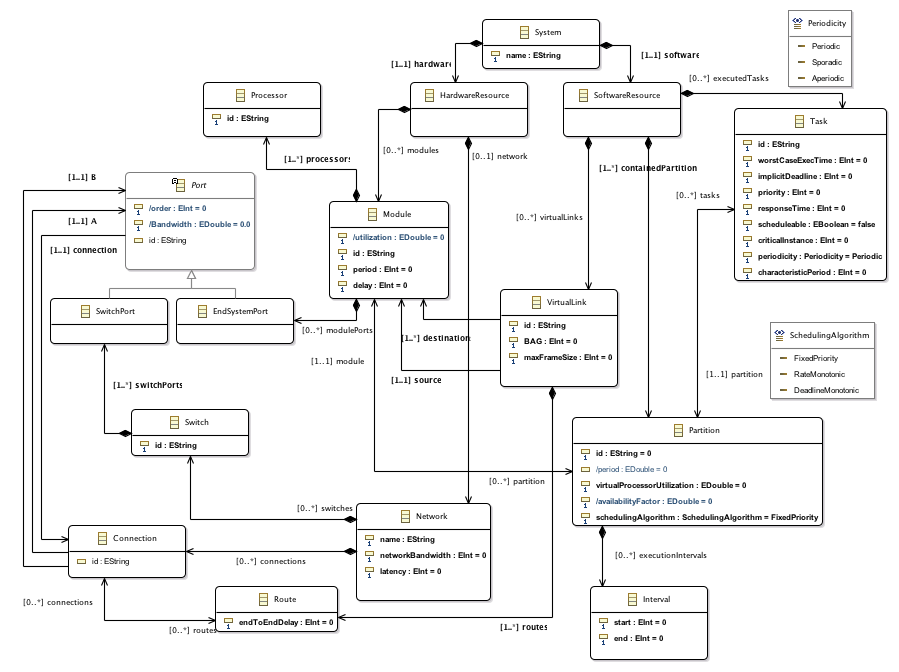
\includegraphics[width=0.8\textwidth]{metamodel_full.png}
    \caption{Full UML meta-model}
    \label{fig:fullmodel} % adding labels for references
\end{figure}

% Now all of the model elements
\paragraph{System}
The root object for an instance of the meta model. This class
serves to hierarchically organize the rest of the classes.
\begin{lstlisting}[caption=System constraints]
class System {
    property hardware : HardwareResource { composes };
    attribute name : String;
    property software : SoftwareResource { composes };
}
\end{lstlisting}

\paragraph{Hardware and Software Resources}
These two classes hierarchically organize other model elements.
\begin{lstlisting}[caption=Hardware and Software constraints]
class SoftwareResource {
    property executedTasks : Task[*] { ordered composes  };
    property containedPartitions : Partition[+] { ordered composes  };
    property virtualLinks : VirtualLink[*] { ordered composes  };
}
class HardwareResource {
    property modules : Module[*] { ordered composes  };
    property network : Network[?] { composes  };
}
\end{lstlisting}

\paragraph{Task}
A task is a software service that has well defined temporal activation parameters.
\begin{lstlisting}[caption=Task constraints]
class Task {
    attribute id : String { id  };
    attribute worstCaseExecTime : ecore::EInt = '0';
    attribute implicitDeadline : ecore::EInt;
    attribute priority : ecore::EInt;
    attribute responseTime : ecore::EInt;
    attribute scheduleable : Boolean;
    attribute criticalInstance : ecore::EInt;
    attribute periodicity : Periodicity = 'Periodic';
    attribute characteristicPeriod : ecore::EInt;
    property partition#tasks : Partition;
    invariant PositiveWCET: worstCaseExecTime > 0;
    invariant ExecutionAndDeadlineAllowsCompletion:
        worstCaseExecTime <= implicitDeadline;
    invariant ExecutionAndPeriodAllowsCompletion: 
        if (periodicity <> Periodicity::Aperiodic)
            then worstCaseExecTime <= characteristicPeriod
        else true
            endif;
    invariant DeadlineLessThanPeriod: implicitDeadline <= characteristicPeriod;
    invariant PositivePeriod: characteristicPeriod > 0;
}
\end{lstlisting}
\paragraph{Constraint Details} 
\begin{description}
    \item[\texttt{PositiveWCET}] The worst case execution time of a task must be a positive number.
    \item[\texttt{ExecutionAndDeadlineAllowsCompletion}] The WCET must be less than or equal to the implicit deadline otherwise the task will never complete in time.
    \item[\texttt{ExecutionAndPeriodAllowsCompletion}] The WCET must be less than or equal to the period of the task. This is only a constraint on \textit{aperiodic} tasks: tasks without a minimum time between arrivals.
    \item[\texttt{DeadlineLessThanPeriod}] The deadline of the task must be less than or equal to the period otherwise multiple instances of the task will exist simultaneously.
    \item[\texttt{PositivePeriod}] The period of a task must be a positive number.
\end{description}

\subsection{Complex Validation}
